\documentclass[conference]{IEEEtran}

\IEEEoverridecommandlockouts
\usepackage{cite}
\usepackage{amsmath,amssymb,amsfonts}
\usepackage{algorithmic}
\usepackage{graphicx}
\usepackage{textcomp}
\usepackage{xcolor}
\usepackage{fancyhdr}
\usepackage{lipsum}

\def\BibTeX{{\rm B\kern-.05em{\sc i\kern-.025em b}\kern-.08em
    T\kern-.1667em\lower.7ex\hbox{E}\kern-.125emX}}
    
\fancypagestyle{firstpagefooter}{%
  \fancyhf{}
  \renewcommand\headrulewidth{0pt}
  \fancyfoot[R]{Sporadic Server, Hamm-Lippstadt Hochschule}
}

\pagestyle{empty}

\bibliographystyle{IEEEtran}

\begin{document}
\title{Sporadic Server}

\author{\IEEEauthorblockN{Vytaras Juraska}
\IEEEauthorblockA{\textit{Electronics Engineering (6\textsuperscript{th} Semester)} \\
\textit{Hamm-Lippstadt Hochschule}\\
Lippstadt, Germany \\
vytaras.juraska@stud.hshl.de}
}

\maketitle

\begin{abstract}
an explanation and a deep dive on the working concept and the mathematical definition of an aperiodic task scheduling approach - called Sporadic Server. 
\end{abstract}
    

%\begin{IEEEkeywords}
%component, formatting, style, styling, insert
%\end{IEEEkeywords}

\thispagestyle{firstpagefooter}

\section{Introduction}
All around of us there are many various real-time systems just silently running in the background without us even being aware of them. For example, flight control and defence systems, that have respectable time constraints, which are responsible for the insured functionality of many various sensors, of which the validity of data is crucial. Further more, there are many services used by us daily, which need to ensure the Quality of Service (QoS), for a smooth and pleasant experience, for instance streaming applications, video games, entertainment systems and so on.

Real-time workloads are known to need predictability, to ensure quality and reliability and in reality, there are many ways of scheduling these workloads, since typically a task is periodic, predictable, has a lot of properties, which help managing priorities of scheduling and understanding the required steps to manage tasks with limited computational power and other resources. But what would happen, if our task would lose a lot of its properties, which provide predictability? Well, Sporadic Server approach is a unique solution to this unique problem. 

But first of all, it is better to have a more detailed definition of the type of the task, which is causing the change in the scheduling solution.

\section{Sporadic/Aperiodic Tasks}

Usually periodic tasks consist of an infinite sequence of identical activities, which are called instances or jobs and are activated at a constant frequency. Taking a look at the \textbf{Figure \ref{tasks}} we can see various notations, which belong to periodic tasks (a). In order to understand these tasks, it is useful to go through its typical variables, which are used in any scheduling algorithm to perform from basic to more complex operations.

The periodic task is noted as $\tau_i$, where as ordinary instance is noted as $k$, hence the periodic job is $\tau_{ik}$. Once the first instance begins ($\tau_{i,1}$), typically the period of that instance beginning is called a \textit{phase}, which is noted as $\phi_i$. So, if $\phi_i$ is a \textit{phase} of a task $\tau_i$, the activation time of the instance $k$ is given by $\phi_i + (k-1)T_i$, where in this case $T_i$ is the activation \textit{period} of a task. Usually, since a periodic task is predictable, the main variables, with which it is possible to characterise the whole process are its phase $\phi_i$, its computational time $C_i$, its period $T_i$ and its relative deadline $D_i$.

Sporadic/Aperiodic Task - a very hectic and unpredictable task: arrival times are unknown, execution times might be also unknown. To understand what kind of solution should be applied we should understand the worst case scenario of this specific task, since if we can handle the worst, we can handle any type of aperiodic task. So the characteristics of a hardest to schedule aperiodic task are:

\begin{itemize}
    \item Minimum time between arrivals of each task, high frequency;
    \item Having a known deadline, which would have the highest priority, the requirement of running the task until completion.
\end{itemize}

These characteristics define an aperiodic task, which is called - sporadic.

Looking back at the \textbf{Figure \ref{tasks}}, aperiodic task is defined as $J_i$, as we can see, it has one of the main variables similar to periodic task, the only difference is that since its jobs are not periodic, each job arrival time $a_{ik}$ and its absolute deadline $d_{ik}$ are defined separately.

\begin{figure}[htbp]
\centerline{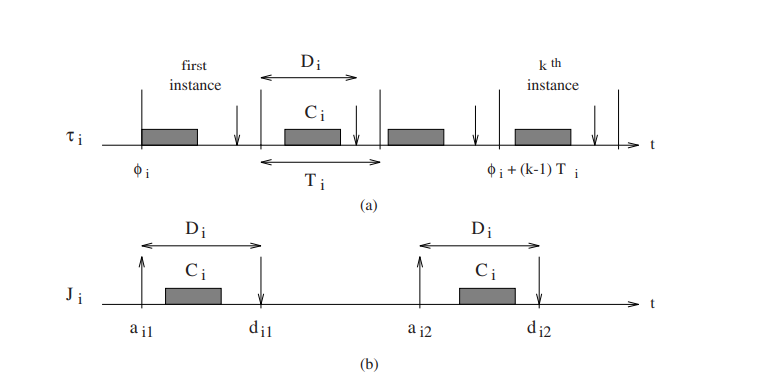
\includegraphics[scale=.48]{Tasks.png}}
\caption{Sequences of (a) Periodic Tasks and (b) Aperiodic Tasks \cite{b1}}
\label{tasks}
\end{figure}

Hence, over all the periodic and aperiodic tasks have similar variables, the only difference, is that arrival and absolute deadline times on a periodic task are defined in a more general way, having an easily predictable definition of each instance, whereas aperiodic tasks have a separate variable for each instances arrival and deadline, has much less predictability, in theory - very hard to schedule.

A sporadic tasks are aperiodic tasks with a couple of more additions to their characteristics, which makes the tasks even more so unpredictable, hard to schedule. The differences are as follows:

\begin{itemize}
    \item The minimum separation between two consecutive instances in a sporadic tasks can't be equal to zero, while on aperiodic tasks instances can come one right after the other;
    \item Sporadic tasks have a hard deadline, meaning a failure of a sporadic task may lead to complete system failure, where as aperiodic task have a soft deadline - the failure of aperiodic tasks are less severe.
\end{itemize}

Hence, sporadic and aperiodic tasks are not to be confused, but they have a lot of similarities between them, although in this case we will be focusing more on the aperiodic tasks.

\section{Sporadic Server}
The Sporadic Server (SS) algorithm is a technique, proposed by Sprunt, Sha, and Lehoczky, which improves the average response time of aperiodic tasks without disregarding the utilisation bound of the periodic tasks. Throughout the whole section of SS a book of Giorgio C. Buttazzo about hard real-time systems will be the main reference point \cite{b1}.

Basic explanation of the working principle, is that SS creates a high-priority task for servicing aperiodic tasks and preserves the server capacity at its high-priority level until aperiodic event occurs. Now this concept is not necessarily unique, it is also applicable to a couple of already existent server algorithms (for instance, a similar concept applies to Deferrable Server and Priority Exchange algorithm), but the biggest key difference with SS, is the way it replenishes its capacity - while others replenish its fully capacity at the beginning of each server period, SS replenishes its capacity only after it has been consumed by aperiodic task execution.

In order to simplify the explanation of working concept of SS algorithms replenishment method, following terms are defined:

\begin{itemize}
    \item $P_{exe}$ Priority level of the task, which is being currently executed;
    \item $P_s$ Priority level associated with the SS;
    \item \textbf{Active} SS is said to be \textit{active}, when $P_{exe} \geq P_s$;
    \item \textbf{Idle} SS is said to be \textit{idle}, when $P_{exe} < P_s$;
    \item \textbf{RT} \textit{Replenishment time} at which the SS capacity will be replenished;
    \item \textbf{RA} \textit{Replenishment amount} that will be added to the capacity at the end of the \textbf{RT};
\end{itemize}

Having these properties defined, we can start estimating the amount of capacity $C_s$ consumed by aperiodic requests according to the following rules:

\begin{itemize}
    \item The replenishment time \textbf{RT} is set as soon as SS becomes active and $C_s > 0$, let's define $t_A$ to be such a time. The value of \textbf{RT} is set equal to $t_A$ plus the server period $(\textbf{RT} = t_A + T_s)$;
    \item  replenishment amount \textbf{RA} has to be done at the time of \textbf{RT} and is computed, when SS be comes idle or $C_s$ has been exhausted, let's call this specific time as $t_I$. The value of \textbf{RA} is set equal to the capacity consumed within the interval $[t_A, t_I]$;
\end{itemize}

Hence, knowing these specific rules and properties defined we can apply this to an exercise of SS scheduling. Taking a look at specific scenarios, SS has a few alternative working principles, according to its priority.

\subsection{Medium-Priority Sporadic Server Example}

\begin{figure}[htbp]
\centerline{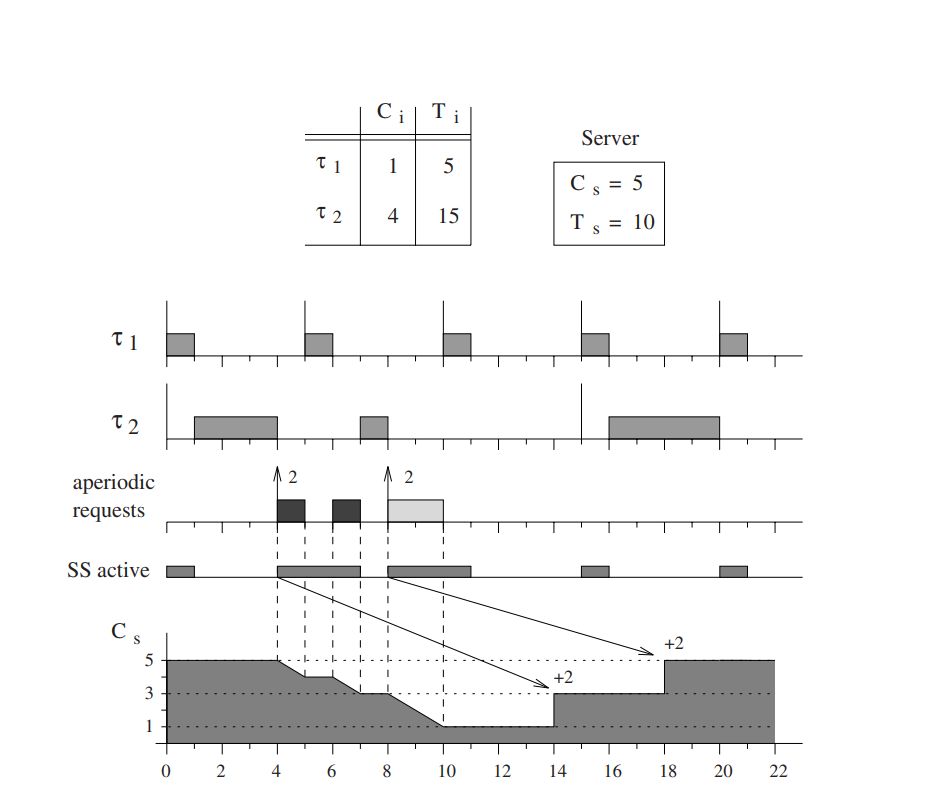
\includegraphics[scale=.38]{Example1.png}}
\caption{Medium-Priority Sporadic Server \cite{b1}}
\label{example1}
\end{figure}

An example of medium-priority SS scheduling is shown in the \textbf{Figure \ref{example1}}. In this example we have a couple of periodic tasks, together with some aperiodic tasks appearing in the scheduling, while we have a limited supply of just 1 processor. Here we can also see the interval of when the SS is active, just to give a better understanding of how the replenishment rule functions.

At time of $t = 0$, the highest priority task $\tau_1$ is scheduled, and SS becomes active. Since the $C_s > 0$, applying the first rule, a replenishment is set at the time of $RT_1 = t + T_s = 0 + 10 = 10$. At time $t = 1$, $\tau_1$ finishes execution, and since no aperiodic tasks are pending, the SS becomes idle. So far the $RT_1 = 10$, while $RA_1 = 0$, since no aperiodic tasks appeared, no replenishment happened and our capacity remains as it was before.

Further on continuing, the scheduler starts $\tau_2$ task and successfully continues executing it, until $t = 4$, where the SS abruptly becomes active, and since $C_s > 0$, SS immediately allows the first aperiodic task $J_1$ to take over the processing unit. After a sudden abruption, the replenishment is set $RT_2 = t + T_s = 4 + 10 = 14$. Sequentially, $J_1$ is abrupted by the periodic $\tau_1$ task at $t = 5$, at $t = 6$ $J_1$ is continued again, where one $t$ later it is finished. Since for $J_1$ to begin, $\tau_2$ finishes its execution, ending at $t = 8$. At this time, the amount of replenishment, which is already done at the replenishment time of $RT_2$ is set equal to the capacity consumed in the interval of $[4,7]$, which is $RA_2 = 2$, hence after the $J_1$ task, our $C_s = 3$.

Paying attention at the SS activation, we can see, that even if the aperiodic task has been executed with discontinuous service, throughout the whole interval of $J_1$ execution, SS stayed active.

To finish off with this example, at the time of $t = 8$, SS becomes active again and a new replenishment is set $RT_3 = t + T_s = 8 + 10 = 18$, a new aperiodic task begins its execution, and since there are no other tasks interfering with the current execution, it ends at $t = 10$. Since the current aperiodic task used up 2 $t$ slots, the replenishment needed to be done is $RA_3 = 2$. Continuing further, periodic tasks are being executed without abruption, while the capacity replenishes at the $t = 14$ and $t = 18$, increasing the $C_s$ by exactly 2 each time, which would be equivalent to each of the aperiodic task execution times.

To sum the example up, SS operated as expected, but since it had medium priority, the tasks, which had the top priority, in this case $\tau_1$, had to be executed at all costs, even having to abrupt $J_1$ in the middle of its execution, while also using the SS activation each time the $\tau_1$ is being called, just to not have aperiodic tasks interrupting the task. Hence, this is an implementation of medium-priority SS.

\subsection{High-Priority Sporadic Server Example}

\begin{figure}[htbp]
\centerline{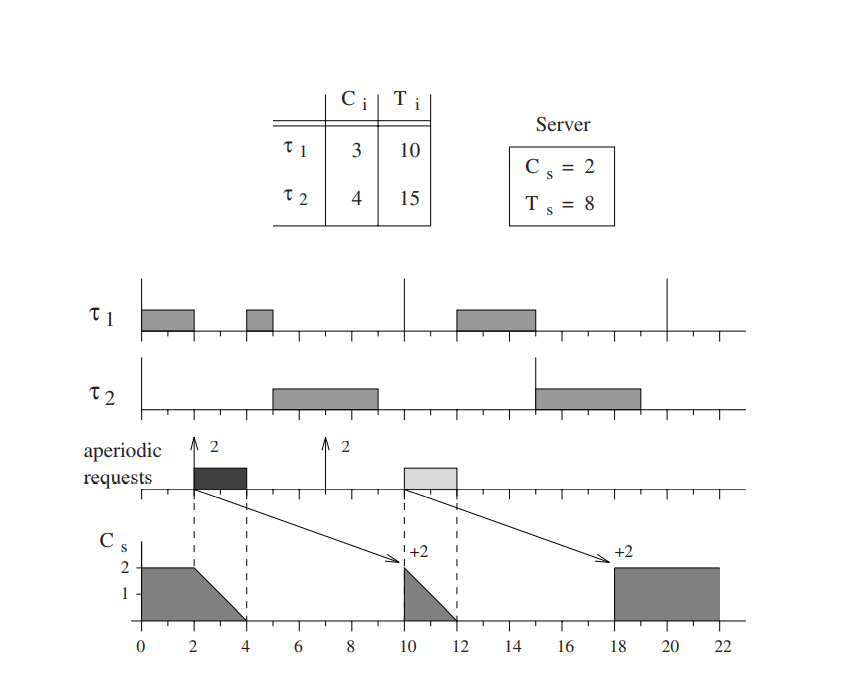
\includegraphics[scale=.39]{Example2.png}}
\caption{High-Priority Sporadic Server \cite{b1}}
\label{example2}
\end{figure}

Taking a look at the \textbf{Figure \ref{example2}}, it shows an example of a high-priority SS scheduling. Here, similar to the previous example, we have two periodic tasks continuously running, while also having a few of high-priority aperiodic tasks appearing in the scheduling. As previously, this task is also restricted to just a single processing unit. Although in this example there is no more visualisation of SS activation, since in this example its functionality does not differ.

Focusing on the aperiodic tasks, the first one $J_1$ starts at the time of $t = 2$, interrupting the $\tau_1$, since at this example SS has high-priority. Without any possible abruptions the $J_1$ ends at $t = 4$, and since it took 2 $t$ slots, its $RA_1 = 2$. Taking a look at servers $C_s$, after the $J_1$ it becomes absolutely empty. Calculating the $RT_1 = t + T_s = 2 + 8 = 10$, makes it clear, that the server will only replenish at $t = 10$.

Continuing further with the example, at $t = 7$ another aperiodic task $J_2$arrives, but since at the arrival time $C_s = 0$, the task has to wait for the execution until the capacity replenishes. And so at $t = 10$, once the capacity rises up again to 2, $J_2$ task abrupts the $\tau_1$ task, executes without any issues and drains the server capacity again, leaving the server to wait for the $RT_2 = t + T_s = 10 + 8 = 18$, until it will replenish and will be able to execute future upcoming aperiodic tasks again.

Summing up the example of high-priority SS scheduling, we can see, that once the aperiodic tasks arrives, the only property which can delay the task is the server capacity and the time it requires to replenish. Other than that, both medium-priority and high-priority function relatively the same way.

\section{Reinterpretation}

There is a unique way to define the concept of SS, differently from previous definitions. From a scheduling point of view, we can treat SS as a periodic task with a period $T_s$ and execution time $C_s$. The theory is as follows: "A periodic task set that is schedulable with a task $τ_i$ is also schedulable if $τ_i$ is replaced by a Sporadic Server with the same period and execution time." \cite{b1}

This is easily proved by showing, that for any type of service - SS execution can be represented by one or more periodic tasks. Let's define $t_A$ as a time at which the previously defined server capacity $C_s$ is filled and SS turns to an active state, and on the contrary, let's say that $t_I$ is the time, when SS is idle, hence the period, of when SS is active is represented by $[t_A,t_I ]$.  Using the method of delaying a periodic task, this characteristic can be simply defined in three unique cases.

\subsection{Full Server Capacity}

If during the $[t_A,t_I ]$ period SS capacity does not get consumed, no replenishments will be done until $t_I + T_s$, which means, that all of the server capacity $C_s$ can be executed in the period of  $[t_A,t_I  + T_s]$. Theoretically, in this scenario we can replace SS with a periodic task, which we can call $\tau_s$, where its computational time would be $C_s$ and its period would be $T_s$ and it simply had a delay time from $t_A$ to $t_I$. Theoretically, if a periodic task is delayed, it will not affect other periodic tasks (the delay is easily dealt with in an algorithm, called Rate Monotonic Scheduling). This behaviour is visualised in the Figure \ref{rein1}

\begin{figure}[htbp]
\centerline{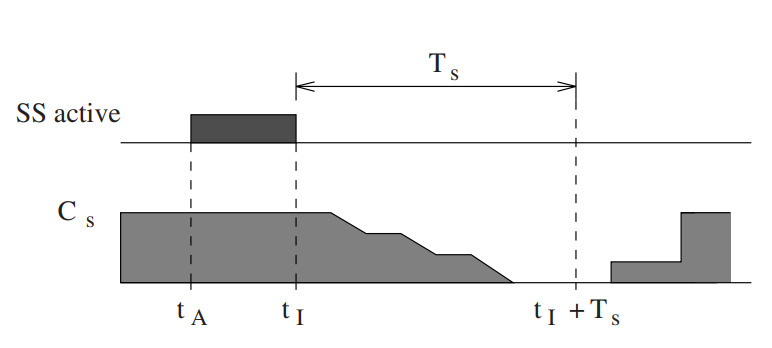
\includegraphics[scale=.39]{reinterpretation_full_capacity.png}}
\caption{SS Server Capacity is Full \cite{b1}}
\label{rein1}
\end{figure}

\subsection{Empty Server Capacity}

If the SS server capacity gets fully consumed at the period of  $[t_A,t_I ]$, then a replenishment will happen at the time of $t_A + T_s$. This is an exact behaviour of a simple periodic task, with the computational time of $C_s$ and period of $T_s$, no delay of the tasks release has to be done. Figure \ref{rein2} displays mentioned behaviour.

\begin{figure}[htbp]
\centerline{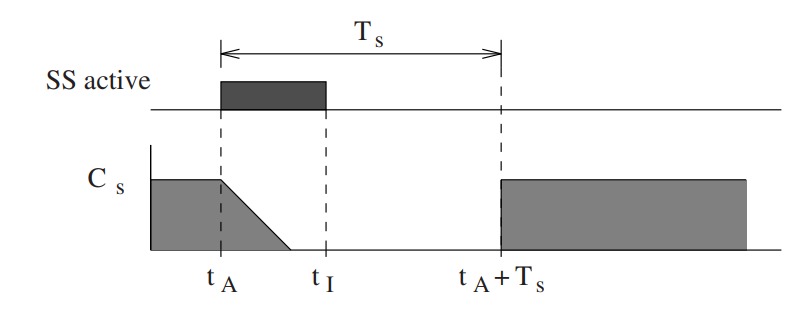
\includegraphics[scale=.39]{reinterpretation_no_capacity.png}}
\caption{SS Server Capacity is Empty \cite{b1}}
\label{rein2}
\end{figure}

\subsection{Partial Server Capacity}

If the SS server capacity is partially used up in the period of  $[t_A,t_I ]$, then a replenishment is needed at $t_A + T_s$. This  reinterpretation would be done defined using two periodic tasks, having the same period, the only characteristic differentiating these tasks would be computational time. Defining, that $C_R$ is the server capacity consumed at the period of $[t_A,t_I ]$, we could define the other periodic tasks computational time as $C_s - C_R$. Hence this behaviour can be reinterpreted as a periodic task $\tau_x$ with computational time $C_x = C_R$ and period $T_x = T_s$ and as a second periodic task $\tau_y$ with computational time $C_y = C_s - C_R$ and period $T_y = T_s$. In the Figure \ref{rein3} a visualisation of this exact scenario is represented.

\begin{figure}[htbp]
\centerline{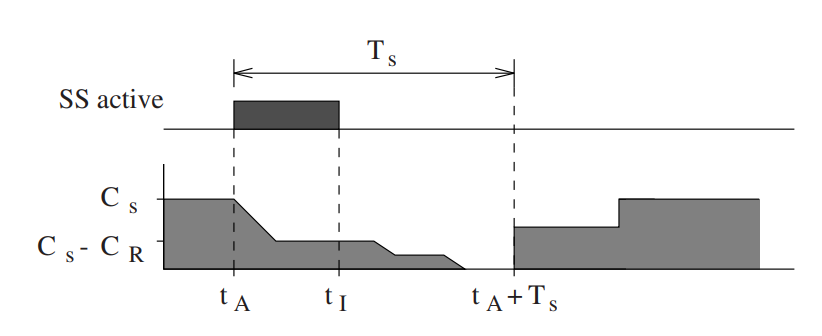
\includegraphics[scale=.39]{reinterpretation_partial_capacity.png}}
\caption{SS Server Capacity is Partially Used \cite{b1}}
\label{rein3}
\end{figure}

\section{Advantages}
Of course, the main advantage of using the SS implementation of aperiodic task scheduling, is that even if we take out one of the most helpful properties from a task, which help us easily schedule any task with even the absolute minimum required scheduling power and make the task unpredictable, we can maintain the aperiodic scheduling, while still managing to execute periodic tasks.

SS algorithm introduces prioritising, so if there is a periodic task, which has a higher priority, than the SS, aperiodic tasks will not affect the execution times of these specific tasks. Considering, that it is already a fairly complex scenario of maintaining the schedulability, adapting prioritisation is quite impressive.

One of the most unique additions to aperiodic scheduling, which SS introduces, is its replenishing rule and ability to adapt it uniquely to each periodic scheduling while also considering the budget of server capacity.

Furthermore, the performance of SS is, compared to other aperiodic task scheduling approaches, fairly good, according to many studies \cite{b3}.

\section{Disadvantages}
One of the biggest disadvantages, is that SS violates one of the basic assumptions governing the execution of the standard periodic task. The assumption is, that that once a high-priority periodic task is ready for execution, it executes without abruption, but in the example of high-priority SS, any periodic task, no matter its priority, are instantly abrupted and pushed back, if needed.

Another issue, is that more complex scenarios may introduce a lot of difficulties concerning schedulability analysis \cite{b1}, since the server is implemented in a way, where it is fragmented in a bunch of small pieces, only being usable at certain times and each aperiodic task introduces a unique time stamp, after which a certain amount of server capacity will be restored, according to the rule of replenishment. As a consequence, calculating the time at which a certain aperiodic task will be executed, requires to keep track of all of the replenishments that will occur until the deadline of the task.

\section{Summary and Conclusion}
This paper describes the theoretical and practical definition of the Sporadic Server algorithm - a general algorithm for scheduling medium and high priority aperiodic tasks in real-time systems. 

Essentially, it is a well developed solution, which is widely used and concerning the approach for scheduling aperiodic tasks while still having to deal with periodic tasks. Having an upper hand in performance, compared with other aperiodic scheduling approaches, introducing prioritisation in aperiodic tasks and defining a simple to understand implementation of aperiodic server capacity, it is understandable, why in this day and age standards SS is still concerned as a suitable implementation. 

Although, in terms of schedulability, SS can also be simply interpreted as a periodic task with the implementation of delayed task arrival, which, in some scheduling approaches, is handled without issues. Also, considering the violation of one of the standard periodic task assumptions, SS definitely has room for improvement. 

Nevertheless, considering which scheduling approach has the best performance - really depends on the requirements of the implementation needed to be done. Hence, if the system is already aware of the disadvantages of SS, used in specific applications, this scheduling approach can deliver astonishing performance.

\bibliography{references}

\end{document}
